\section{TP7 Apply the Web instead of working around}
\label{sec:principle-tp7-apply-the-web}

Der moderne Internetbrowser kapselt eine Vielzahl von leistungsfähigen Funktionen des jeweiligen Hostrechner in ein für den Software Entwickler leicht zu verwendendes Interface. Dazu gehört die Integration von systemnahen Komponenten wie \gls{GPU}'s \cite{webgl} genauso wie die Möglichkeit, gleichzeitig mehrere Fenster oder Tabs für die selbe oder verschiedenen Applikationen resp. Internetseite offen zu halten.

Das Hin- und Herspringen zwischen besuchten Seiten mittels Vorwärts- und Zurück-Schaltflächen gehört seit Beginn der Webära zum festen Bestandteil der User Experience im Internet.

In der Vergangenheit gehörten wiederkehrende Umsetzungen von Funktionen wie der Validierung von Formularinhalten zu lästigen, aber nötigen Ärgernissen. Mit der Einführung der neusten Revision 5 des HTML Standards können gerade solche Aufgaben bequem dem Browser \cite{HTML5Forms} überlassen werden

Mit der immer mächtiger werdenden Formatierungssprache CSS und dessen neuster Version 3 sind heute gestalterische Effekte möglich, welche bis vor Kurzem nur mittels umständlicher Einbindung von Grafikdateien (Stichwort Schlagschatten \cite{css-box-shadow} oder Farbverlauf \cite{css-gradient}) möglich waren.

Mit der Richtlinie \emph{TP7} hält Stefan Tilkov Software Entwickler dazu an, die Werkzeuge welche vom Internetbrowser angeboten werden, gewinnbringend zu nutzen.


\subsection*{Geplante Umsetzung}

In der Beispielapplikation sollen gezielt HTML 5 Features verwendet werden:

\begin{itemize}
	\item Semantisch korrekte Tags (\emph{<header>}, \emph{<section>} etc.) \cite{SemanticHTML}
	\item Formularvalidierung \cite{HTML5Forms}
\end{itemize}

Das entstehende, semantisch korrekte HTML Markup soll mit CSS 3 gestaltet werden. Neue Möglichkeiten zur grafischen Darstellung sollen ausgenutzt werden.

Bei der Entwicklung der Front- als auch Backend-Komponente muss zwingend darauf geachtet werden, dass die Verwendung der Browser-Funktionen \emph{Vorwärts}, \emph{Zurück} und \emph{Aktualisieren} zu keinem ungewünschten resp. unerwarteten Verhalten führen (siehe hierzu auch Abschnitt \ref{sec:principle-rp10-browser-controls} ``\nameref{sec:principle-rp10-browser-controls}'').


\subsection*{Konkrete Umsetzung}

Das gerenderte HTML Markup verwendet wie geplant vom HTML 5 Standard eingeführte Funktionen. Quellcode \ref{lst:roomiesMenuHtml} zeigt die Verwendung des \emph{<header>} sowie \emph{<nav>} Tags zur Beschreibung des Applikationsmenüs der Beispielapplikation.

\begin{lstlisting}[language=HTML, caption={Ausschnitt des gerenderten HTML Markups der Menüleiste \emph{roomies}}, label={lst:roomiesMenuHtml}]
<header id="menu">
	<div class="fixed-navigation">
		<nav class="navigation" role="navigation">
			<div class="title-area">
				<a href="/" class="banner" title="Roomies"><h1>Roomies</h1></a>
			</div>
			<section class="nav-section">
				<ul class="left">
						<li>
							<a href="/community/ba-team/tasks" title="Aufgaben">
								<i class="icon-tasks icon-large"></i>
								<span class="item-label"> Aufgaben</span>
							</a>
						</li>
						<!-- ... more items -->
				</ul>
				<!-- ... displaying the facebook profile picture -->
			</section>
		</nav>
	</div>
</header>
\end{lstlisting}

Weiter wurde für das \emph{Fällig bis}-Feld auf der Ansicht \emph{Aufgabe bearbeiten} ein Textfeld vom Typ \emph{date} verwendet. Gerade auf einem Mobile Browser wie \emph{Safari für iPhone} kommt diese Implementation voll zum tragen.

\begin{figure}[H]
	\centering
	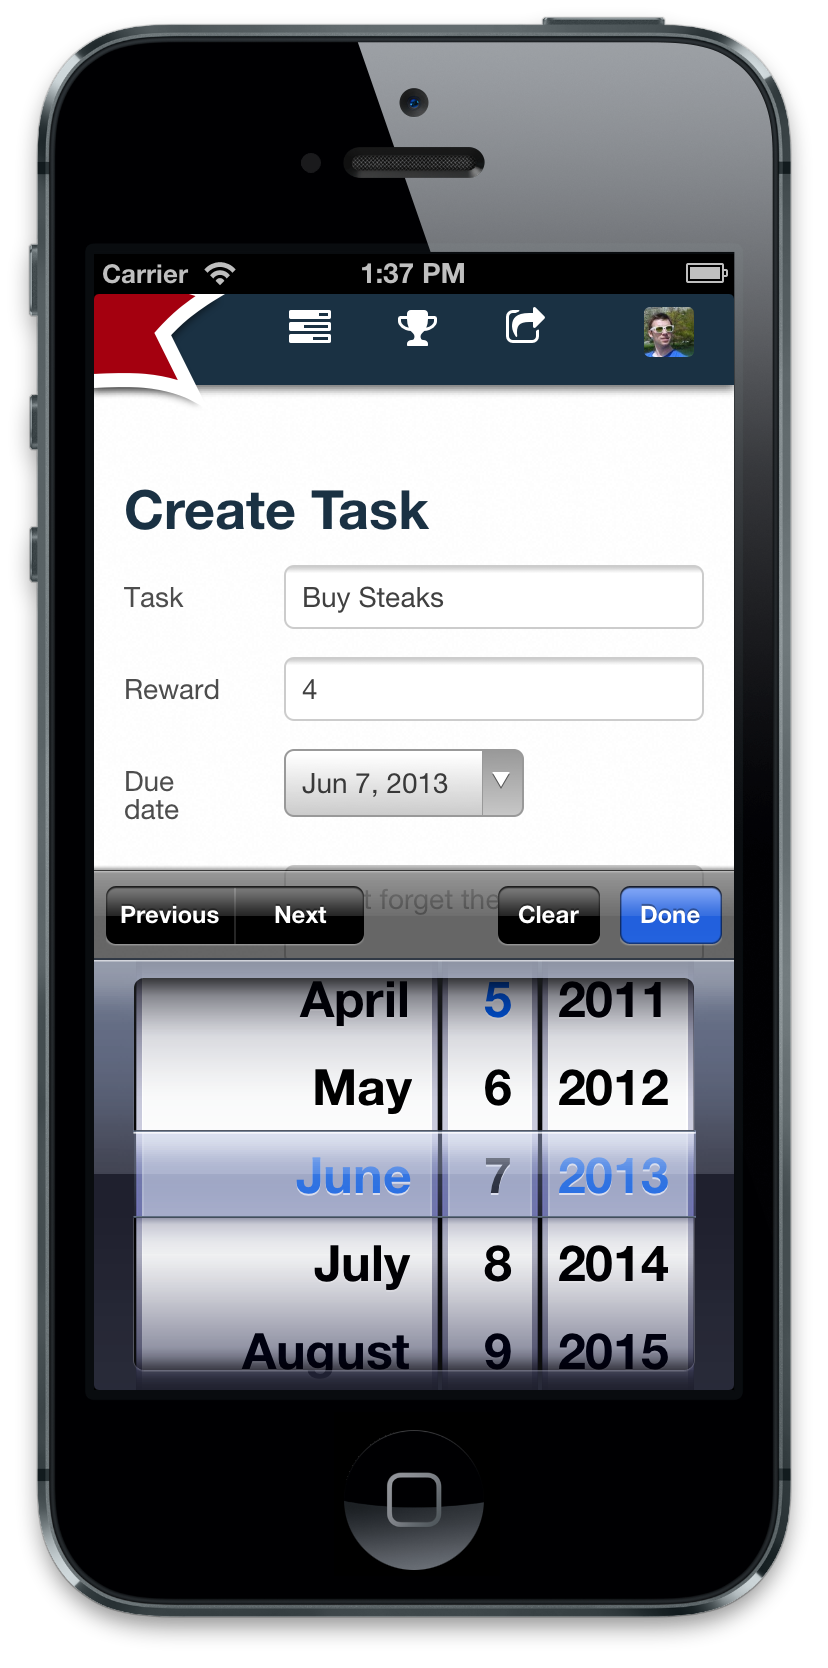
\includegraphics[width=6cm]{content/principle-demonstration/images/iossafari-datepicker.png}
	\caption{Datumsauswahl für ein Textfeld vom Typ \emph{date} in \emph{Safari für iPhone}}
	\label{fig:iossafari-datepicker}
\end{figure}




\subsection*{Diskussion}


